\subsection{Testing}
Testing the modules was done parallel to the implementation of the
respective modules. This made for an incremental work flow that
worked well for a test-driven developing approach for each of the
modules.

\subsubsection{Hazard Detection Unit}
Testing the hazard detection unit was very simple. The unit only
sets output signals for when the pipeline should stall and
if the subsequent instruction should get its input from the 
instruction memory or from the respective instruction.

Because the unit is so simple, the best approach was to create
a test bench with assertions for the different kinds of outputs.
The assertions work as described in Listing \ref{lst:assertion}.

\begin{lstlisting}[caption={Code snippet from the test 
    bench for the hazard detection unit}, label={lst:assertion}]
-- Assert that the pipeline should stall
wait for 4 ns; -- Set input signals
input_id_ex_RegisterRt  <= "00001";
input_if_id_RegisterRs  <= "00001";
input_if_id_RegisterRt  <= "00100";
input_id_ex_MemRead     <= '1';

wait for 1 ns; -- Do assertions on the output signals
assert(output_if_id_write = '0') report "if_id_write = '0'" severity error;
assert(output_pc_write = '0') report "pc_write = '0'" severity error;
assert(output_bubble_op = '1') report "bubble_op = '1'" severity error;
\end{lstlisting}

\subsubsection{Forwarding unit}
The test bench for the forwarding unit was implemented in
the same fashion as the hazard detection unit. 

The test bench proved useful when the code for this
unit was later re-factored and modified during the implementation of the
pipeline itself.

\subsubsection{Synchronizing PC with instruction memory}
One of the greatest concerns for the pipeline was the synchronization 
between the program counter and the instruction memory. Thus we
created a test bench for simulating the behavior between the PC and the
instruction memory, in a closed environment.

The main concern was that the program counter for the PC register and the 
instruction memory updated on the same clock cycle, thus the value of the 
input signal to the
instruction memory are always one clock cycle behind the value of
the input signal to the PC register. An example is show in 
Figure \ref{pc-mem-sync1}. This becomes a problem when current instruction 
is a branch instruction, making the program counters in the different modules
differ by more than 1, an example of this is shown in 
Figure \ref{pc-mem-sync2}.

\begin{figure}[ht]
    \centering
        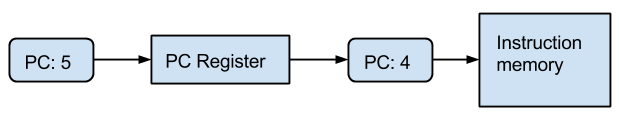
\includegraphics[width=0.6\textwidth]{figures/pc-mem-sync1}
    \caption{Value of PC in PC register and instruction memory, being
    updated when the clock goes high.}
    \label{pc-mem-sync1}
\end{figure}

\begin{figure}[ht]
    \centering
        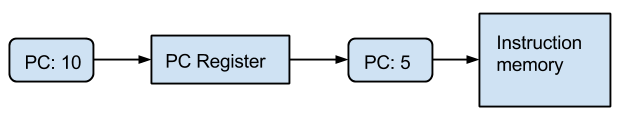
\includegraphics[width=0.6\textwidth]{figures/pc-mem-sync2}
    \caption{Value of PC in PC register and instruction memory when a 
    branch occurs.}
    \label{pc-mem-sync2}
\end{figure}

This problem required an extra no-op in order for the 
instruction memory to get the right program counter when a branch
occurred. The \textbf{pc\_ins\_ mem\_test.vhd} - test bench helped to
manually trace the signals for stalls until we had the desired 
synchronization between the modules.

\subsubsection{Incremental testing of toplevel}
Testing of the toplevel was done in an incremental fashion.
We created the \textbf{tb\_top\_level\_2.vhd}, that started as 
an empty test bench, but ended up very similar to the already
supplied test bench \textbf{tb\_toplevel.vhd}.

The first thing that needed to work was \textbf{load} and 
\textbf{store} instructions. These two instructions in combination
with an arithmetical instruction (e.g. \textbf{add}) made for a natural
starting point.

\begin{figure}[ht]
    \centering
        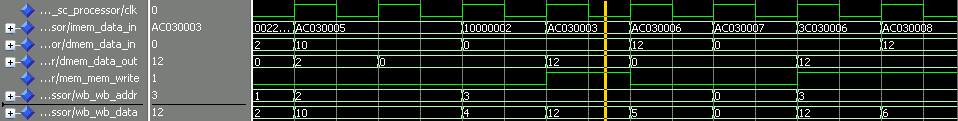
\includegraphics[width=1\textwidth]{figures/sim-load-store-add}
    \caption{Simulation of load(2), load(10), add(2+10) and 
    store of result(12).}
    \label{sim-load-store-add}
\end{figure}

The simulation for this part of the test bench is shown in Figure
\ref{sim-load-store-add}. This simulation includes signals for the
address in instruction memory, the data going in and out of the
data memory and where the write back occurs.

The test bench was extended when the modules gave satisfying results,
in the end test bench simulated the instructions for load, store,
arithmetic results, jumping and branching.

\subsection{Branching}
Because the pipeline predicts branch taken, it sometimes have to 
branch back and continue with the instruction after the branch.

\begin{figure}[ht]
    \centering
        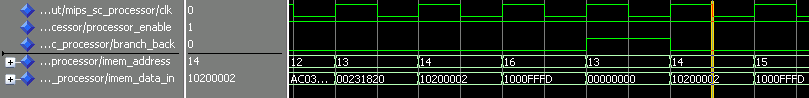
\includegraphics[width=1\textwidth]{figures/branch-back}
    \caption{Simulation of a branch back, after a wrongly predicted
    branch occurs.}
    \label{branch-back}
\end{figure}

Figure \ref{branch-back} shows a simulation of the branch back. Note
that the imem\_address signal is always one step ahead of the 
imem\_data signal.
Instruction 13 is a \textit{branch +2} instruction that compares
R0 with R1, in this case the registers are not equal. Thus it has 
to perform a branch back and continue executing at instruction 14, 
instead of the predicted instruction 16.  Also, keep in mind that 
instruction 13 is bubbled the second time it occurs, and thus it has 
no effect on the program. A branch back like this will result in three
lost clock cycles.

